\section{The Simulation}
In contrast to the large scale threshold analysis done by \citet{OGorman2016} this work focusses on the physical simulation of the building block of the surface code error detection - the stabilizer measurements which is done by measuring the parity of a group of qubits. On the smallest scale this is given by a group of four data qubits and one probe/ancillary qubit as shown in FIG. \ref{FIG:paper-parity}. 

\subsection{The dipole-dipole interaction}

The interaction of the orbiting ancillary qubit with each data qubit is governed by the following Hamiltonian:

\begin{equation*}
H = \mu_B B( g_1 \sigma_1^Z + g_2 \sigma_2^Z) + \frac{J}{r^3} ( \mathbf{\sigma_1} \cdot \mathbf{\sigma_2} - 3 ( \hat{\mathbf{r}} \cdot \mathbf{\sigma_1}) ( \hat{\mathbf{r}}\cdot \mathbf{\sigma_2}))
\end{equation*}

First of all, there is the Zeeman part which accounts for the energy of each spin (data and probe) in an external magnetic field. The interaction is of magnetic dipole-dipole type with the interactions strength $J=\frac{\mu_0 g_e^2 \mu_B^2}{4\pi}$ where $\hat{\mathbf{r}}$ is the unit vector between the two spins. The magnetic dipole-dipole interaction is of long range compared to proposals based on the exchange interaction \cite{Kane1998a} which makes this approach very attractive as it lowers the enormous requirements on the qubit placement precision as shown by \citet{OGorman2016}. Nevertheless, the interaction scales with $1/r^3$ which makes a data to probe qubit distance on the order of several tenths of nanometres necessary to achieve a strong interaction. In order to avoid crosstalk between the data qubits in the plane the lattice spacing $D$ of the data qubits should be at least one order of magnitude larger than the data and probe spacing $d$. 

Our goal is to achieve a parity measurement using this interaction. The dipole-dipole term allows us to do a controlled phase gate between the data and probe qubit which is shown in \cite{OGorman2016} and can be seen from the dependence on both spin matrices $\mathbf{\sigma_1}$ and $\mathbf{\sigma_2}$. This means that depending on the data qubit state the probe qubit in a different direction in the bloch sphere (acquires a different phase). 

In order to simulate the time evolution of both qubits under the effect of this Hamiltonian by solving the Schrödinger or master equation we need to transform into the interaction picture and apply the rotating wave approximation. This allows us to get rid of the fast dynamics given by the Zeeman term while maintaining the physical interaction which we are interested in. 

In this approximation the interaction Hamiltonian is given by:

\begin{align*}
	H_{int}&= \frac{J}{r^3} (1-3 \cdot \hat{r}_z^2) \cdot
	\begin{pmatrix}
	1 & 0 & 0 & 0 \\
	0 & -1 & 0 & 0 \\
	0 & 0 & -1 & 0 \\
	0 & 0 & 0 & 1 
	\end{pmatrix} \\
	&+ \frac{J}{r^3} (2-3 \cdot \hat{r}_x^2 -3 \cdot \hat{r}_y^2) \cdot
	\begin{pmatrix}
	0 & 0 & 0 & 0 \\
	0 & 0 & e^{-4 \Delta i} & 0 \\
	0 & e^{4 \Delta i} & 0 & 0 \\
	0 & 0 & 0 & 0 
	\end{pmatrix}
\end{align*}

Here $\Delta=\mu_B B (g_1-g_2)$. Depending on the relation between $\Delta$ and $J/r^3$ the interaction will have a different character. 
To achieve a controlled phase gate on the probe qubit while keeping the data qubit unchanged we want to be in the regime where $\Delta \gg J/r^3$.
In order to estimate what orders of magnitude we require to achieve this we performed simulations for various magnitudes of $\Delta d^3/ J$.

\begin{figure}[H]
	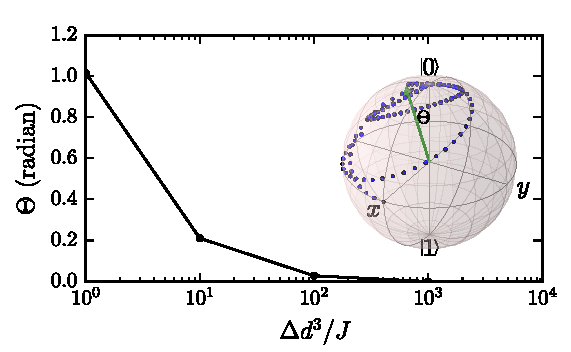
\includegraphics[width=\linewidth]{../Figures/flip-flop}
	\caption{}
	\label{FIG:flip-flop}
\end{figure}

When $\Delta = J/r^3$ we show a strong flip-flopping behaviour between the data (initialised in $\ket{0}$) and probe qubit (initialised in $\ket{+}$) as shown in the inset of FIG. \ref{FIG:flip-flop}. We want to avoid any evolution of the state of the data qubit. To quantify the flip-flopping we plot the angle theta the data qubit evolves for a given time for different magnitudes of $\Delta d^3/ J$ (see FIG. \ref{FIG:flip-flop}). Flip-flopping disappears for $\Delta d^3/ J > 10^4$ preserving the data qubit state. This is achieved by using different species of qubits for the data and probe lattice (see Table. \ref{TAB:qubits}).

\subsection{The parity measurement}
Having identified the regime where the dipole-dipole interaction is able to perform a controlled-phase gate, we move on to the demonstration of a parity measurement.

The parity measurement should report 'even' when the number of data qubits pointing up and pointing down is even. And it should report 'odd' when the number of data qubits pointing up and pointing down is odd.

Realising a parity measurement using the controlled-phase gate is done by initialising the probe qubit in the $\ket{+}$ state and timing the interacting of the probe qubit with every data qubit such that the probe qubit acquires a controlled phase of $\pi/2$ for every data qubit. In case of even parity the probe qubit will then always evolve into the $\ket{+}$ state (see FIG. \ref{FIG:even} for the case of all four qubits being initialised in $\ket{0}$) while odd parity brings the probe qubit to the $\ket{-}$ state (see FIG. \ref{FIG:even} where one of the four qubits has been initialised in $\ket{1}$). The parity is therefore obtained by measuring the probe qubit in the $x$-basis.    


\begin{figure}[H]
	\subfloat[]{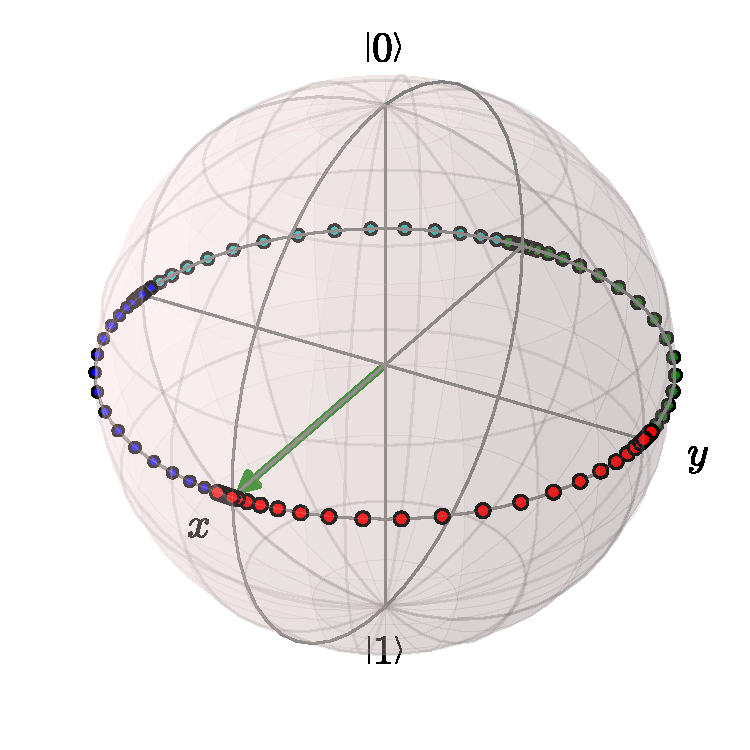
\includegraphics[width=0.49\linewidth]{../Figures/perfect_evolution_even} \label{FIG:even}}
	\subfloat[]{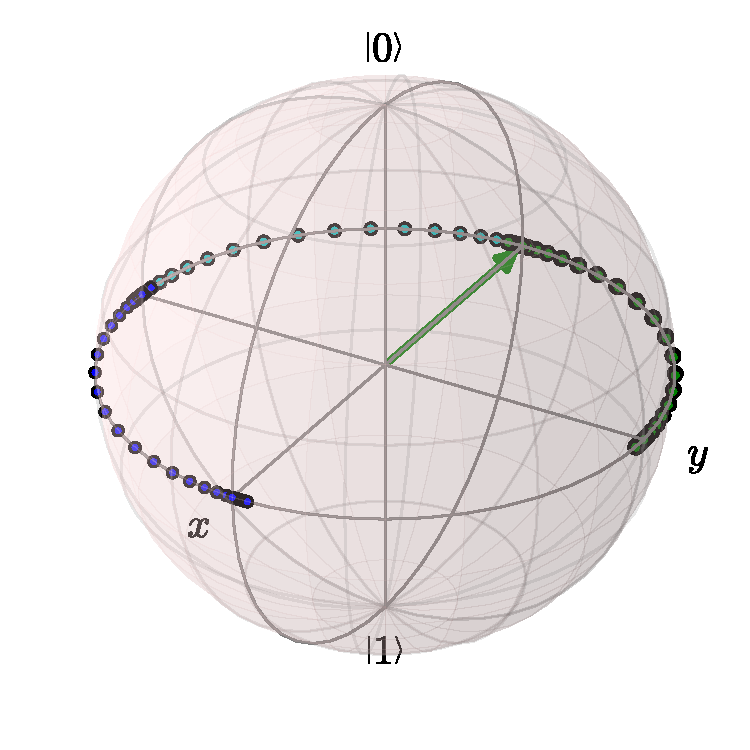
\includegraphics[width=0.49\linewidth]{../Figures/perfect_evolution_odd} \label{FIG:odd}}
	\caption[oddeven]{}
	\label{FIG:evolution}
\end{figure}


The orbit which the probe qubits take to perform the parity measurement can take any possible form. Our simulations include an abrupt movement where the probe qubit jumps directly from one data qubit to the next and so on (see FIG. \ref{FIG:paper-abrupt}). This is very unphysical but describes the optimal orbit as it reduces the parity measurement time to a minimum. In addition to that we simulate a circular orbit with a constant speed (see FIG. \ref{FIG:paper-circ}). In an experiment something between these two extrema will most likely be implemented. 

The time each data qubit should interact with the probe qubit to realise a controlled $\pi/2$ rotation in the bloch sphere is obtained by varying the interaction time while monitoring the phase acquired by the probe qubit. This is done for every chosen orbit and an exemplary simulation is shown in FIG. \ref{FIG:get_tau} for the abrupt orbit. A rotation of $\pi/2$ is achieved for $\tau\approx 77\, \mu$s.

\begin{figure}[H]
	\begin{minipage}[t]{0.15\linewidth} 
	\subfloat[]{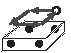
\includegraphics[width=\linewidth]{../Figures/abrupt} \label{FIG:paper-abrupt}}\\
	\subfloat[]{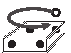
\includegraphics[width=\linewidth]{../Figures/circ} \label{FIG:paper-circ}}
	\end{minipage}
	\subfloat[]{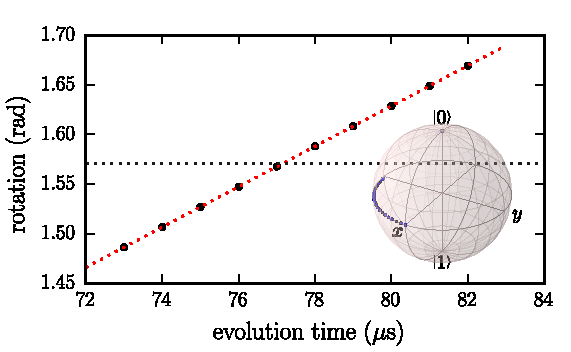
\includegraphics[width=0.85\linewidth]{../Figures/abrupt_find_tau_full.pdf} \label{FIG:get_tau}}
	\caption{}
	\label{FIG:abrupt_tau}

\end{figure}

In order to estimate the time a parity measurement would take in an experiment, we determine the parity measurement time for the abrupt and circular orbit for several data and probe qubit separations $d$ and data qubit lattice spacings $D$.

\begin{figure}[H]
	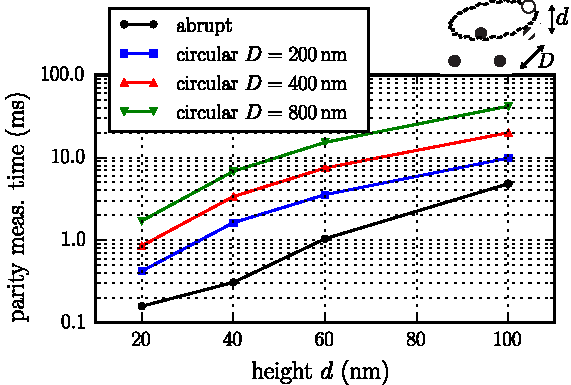
\includegraphics[width=\linewidth]{../Figures/tau_d_D}
	\caption{}
	\label{FIG:tau}
\end{figure}
